\documentclass[xcolor=table]{beamer}
%------------------------------------------------------------
% Theme and Appearance
%------------------------------------------------------------
\usetheme[footline=authorinstitutetitle]{Berlin} 
\setbeamertemplate{navigation symbols}{} 

% Headline with Access Code
\setbeamertemplate{headline}{
    \begin{beamercolorbox}[wd=\paperwidth,ht=2.5ex,dp=1ex,right]{section in head/foot}
        \usebeamerfont{section in head/foot}
        \hspace{0.5cm}
        \ifnum\insertframenumber<30
            \raisebox{-1pt}[0pt][0pt]{\normalsize\textbf{Attendance Code: 930068}}
        \fi
        \hspace{0.5cm}
    \end{beamercolorbox}
}
% Footline with page numbers
\setbeamertemplate{footline}{
    \leavevmode%
    \hbox{%
        \begin{beamercolorbox}[wd=.333333\paperwidth,ht=2.25ex,dp=1ex,left]{author in head/foot}%
            \usebeamerfont{author in head/foot}\hspace*{0.5em}\insertshortauthor
        \end{beamercolorbox}%
        \begin{beamercolorbox}[wd=.333333\paperwidth,ht=2.25ex,dp=1ex,center]{title in head/foot}%
            \usebeamerfont{title in head/foot}\insertshorttitle
        \end{beamercolorbox}%
        \begin{beamercolorbox}[wd=.333333\paperwidth,ht=2.25ex,dp=1ex,right]{date in head/foot}%
            \usebeamerfont{date in head/foot}\insertshortdate{}\hspace*{2em}
            \insertframenumber{} / \inserttotalframenumber\hspace*{2ex} 
        \end{beamercolorbox}}%
    \vskip0pt%
}
\usepackage[utf8]{inputenc}
\usepackage[table]{xcolor}
\usepackage{colortbl}
\usepackage{minted}
\usepackage{lmodern}
\usepackage{tgheros}
\usepackage{hyperref}
\usepackage{tikz}
\usetikzlibrary{shapes, arrows, arrows.meta, positioning, shadows, fit, calc, shapes.multipart, backgrounds}

\renewcommand*\familydefault{\sfdefault}

% Agenda at the start of every section
\AtBeginSection[]
{
    \begin{frame}
        \frametitle{Agenda}
        \tableofcontents[currentsection]
    \end{frame}
}

%------------------------------------------------------------
% Title Page Information
%------------------------------------------------------------
\title[CMP9134 - Week 5]{Software Architecture, Patterns \& Reuse}
\subtitle{CMP9134: Software Engineering}
\author[Francesco Del Duchetto]{Dr Francesco Del Duchetto\\Lecturer in Robotics and Autonomous Systems}
\institute[University of Lincoln]{University of Lincoln}
\date{6 March 2026}

%------------------------------------------------------------
\begin{document}

%--- TITLE FRAME ---
\begin{frame}
    \titlepage
\end{frame}

%--- AGENDA FRAME ---
\begin{frame}
    \frametitle{Today's Agenda}
    \tableofcontents
\end{frame}

%------------------------------------------------------------
\section{Recap: Week 4}
%------------------------------------------------------------

\begin{frame}
    \frametitle{Recap: System Modelling \& UML}
    Last week, we explored how to abstract our system requirements into visual models.
    
    \begin{itemize}
        \item \textbf{Use Case Diagrams:} External perspective (Actors and their goals).
        \item \textbf{Sequence Diagrams:} Interaction perspective over time (Lifelines and Messages).
        \item \textbf{Class Diagrams:} Structural perspective (OOP Encapsulation, Inheritance, Aggregation vs Composition).
        \item \textbf{Activity Diagrams:} Behavioral perspective (Flow of control, forks, and decisions).
    \end{itemize}
\end{frame}

\begin{frame}
    \frametitle{Today's Learning Objectives}
    By the end of this lecture, you should be able to:
    \begin{enumerate}
        \item \textbf{Differentiate} between high-level Architectural Patterns and low-level Design Patterns.
        \item \textbf{Identify} common architectural patterns like Layered and Model-View-Controller (MVC).
        \item \textbf{Apply} standard GoF Design Patterns (e.g., Singleton, Observer) to solve recurring coding problems.
        \item \textbf{Evaluate} the benefits and risks of Software Reuse and Open Source licensing in modern engineering.
    \end{enumerate}
\end{frame}

%------------------------------------------------------------
\section{Architectural Patterns}
%------------------------------------------------------------

\begin{frame}
    \frametitle{What is an Architectural Pattern?}
    \begin{block}{Definition}
        Patterns are a means of representing, sharing, and reusing knowledge about a commonly occurring problem in software architectures.
    \end{block}
    \vspace{0.3cm}
    \textbf{Why use them?}
    \begin{itemize}
        \item They provide a stylized description of good design practice that has been tried and tested.
        \item Architecture heavily dictates performance, robustness, and distributability.
        \item It enhances stakeholder communication (e.g., "We are using a Client-Server model").
    \end{itemize}
\end{frame}

\begin{frame}[fragile]
    \frametitle{Pattern 1: Layered Architecture}
    Organizes the system into a set of layers, each providing a set of services to the layer above it.
    
    \vspace{0.3cm}
    \centering
    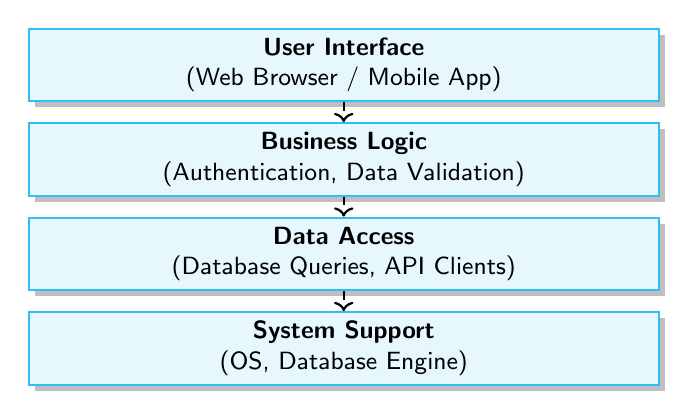
\begin{tikzpicture}[
        layer/.style={rectangle, draw=cyan!80, fill=cyan!10, thick, minimum width=8cm, minimum height=0.8cm, align=center, font=\small, drop shadow}
    ]
        \node[layer] (ui) at (0,3) {\textbf{User Interface}\\(Web Browser / Mobile App)};
        \node[layer] (biz) at (0,1.8) {\textbf{Business Logic}\\(Authentication, Data Validation)};
        \node[layer] (data) at (0,0.6) {\textbf{Data Access}\\(Database Queries, API Clients)};
        \node[layer] (db) at (0,-0.6) {\textbf{System Support}\\(OS, Database Engine)};
        
        \draw[->, thick, dashed] (ui.south) -- (biz.north);
        \draw[->, thick, dashed] (biz.south) -- (data.north);
        \draw[->, thick, dashed] (data.south) -- (db.north);
    \end{tikzpicture}
    
    \vspace{0.2cm}
    \footnotesize \textit{Advantage: You can replace an entire layer (e.g., swapping a web UI for a mobile UI) without affecting the core business logic.}
\end{frame}

\begin{frame}[fragile]
    \frametitle{Example: Library System Layered Architecture}
    \vspace{0.3cm}
    \centering
    \resizebox{0.9\textwidth}{!}{
    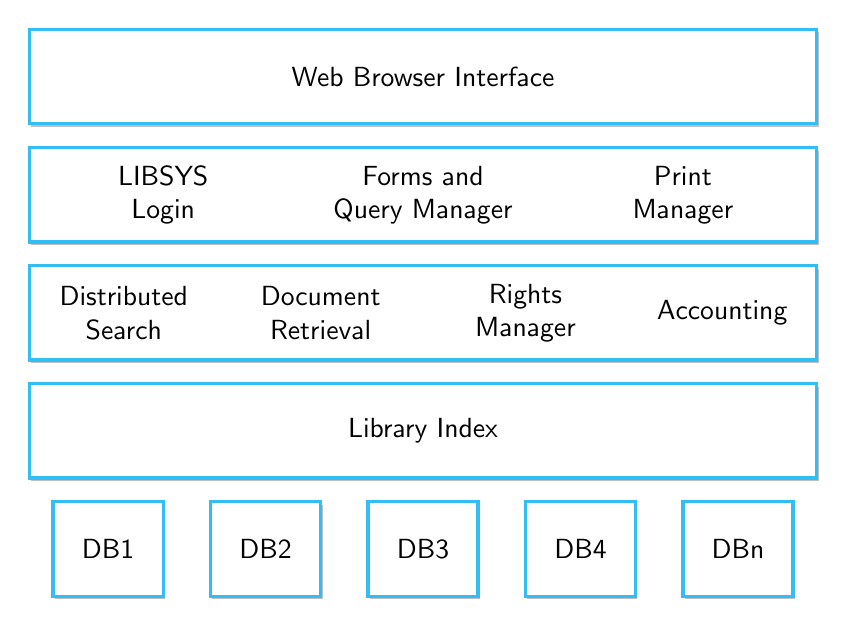
\begin{tikzpicture}[
        layer/.style={rectangle, draw=cyan!80, fill=white, very thick, minimum width=10cm, minimum height=1.2cm, align=center, drop shadow={shadow xshift=0.15ex, shadow yshift=-0.25ex}},
        db/.style={rectangle, draw=cyan!80, fill=white, very thick, minimum width=1.4cm, minimum height=1.2cm, align=center, drop shadow={shadow xshift=0.15ex, shadow yshift=-0.25ex}}
    ]
        % Layer 1
        \node[layer] (l1) at (0, 6) {Web Browser Interface};
        
        % Layer 2
        \node[layer] (l2) at (0, 4.5) {};
        \node[align=center] at (-3.3, 4.5) {LIBSYS\\Login};
        \node[align=center] at (0, 4.5) {Forms and\\Query Manager};
        \node[align=center] at (3.3, 4.5) {Print\\Manager};
        
        % Layer 3
        \node[layer] (l3) at (0, 3) {};
        \node[align=center] at (-3.8, 3) {Distributed\\Search};
        \node[align=center] at (-1.3, 3) {Document\\Retrieval};
        \node[align=center] at (1.3, 3) {Rights\\Manager};
        \node[align=center] at (3.8, 3) {Accounting};
        
        % Layer 4
        \node[layer] (l4) at (0, 1.5) {Library Index};
        
        % Layer 5
        \node[db] (db1) at (-4, 0) {DB1};
        \node[db] (db2) at (-2, 0) {DB2};
        \node[db] (db3) at (0, 0) {DB3};
        \node[db] (db4) at (2, 0) {DB4};
        \node[db] (dbn) at (4, 0) {DBn};
    \end{tikzpicture}
    }
\end{frame}

\begin{frame}[fragile]
    \frametitle{Pattern 2: Model-View-Controller (MVC)}
    Separates presentation and interaction from the system data. Highly standard for Web Applications.
    
    \vspace{0.2cm}
    \begin{center}
    \resizebox{0.8\textwidth}{!}{
    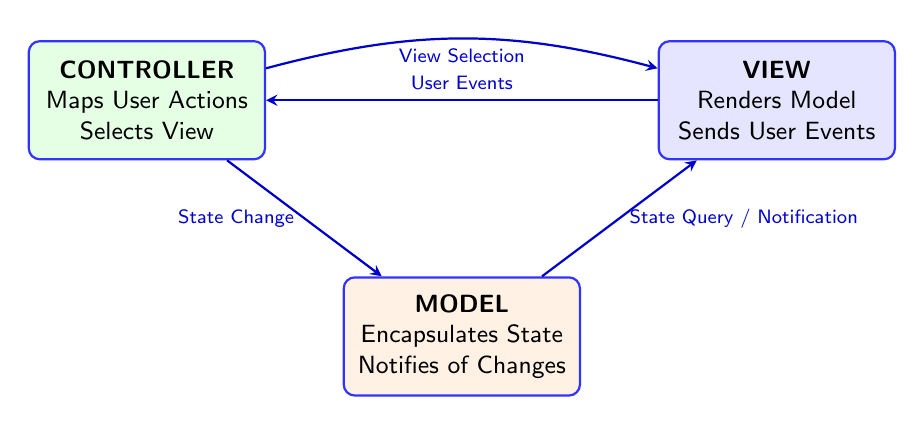
\begin{tikzpicture}[
        box/.style={rectangle, draw=blue!80, fill=white, thick, minimum width=3cm, minimum height=1.5cm, align=center, rounded corners, font=\small},
        arrow/.style={->, >=stealth, thick, blue!80!black}
    ]
        \node[box, fill=blue!10] (view) at (4, 3) {\textbf{VIEW}\\Renders Model\\Sends User Events};
        \node[box, fill=green!10] (ctrl) at (-4, 3) {\textbf{CONTROLLER}\\Maps User Actions\\Selects View};
        \node[box, fill=orange!10] (model) at (0, 0) {\textbf{MODEL}\\Encapsulates State\\Notifies of Changes};
        
        \draw[arrow] (view) -- node[above, font=\scriptsize] {User Events} (ctrl);
        \draw[arrow] (ctrl) -- node[left, font=\scriptsize] {State Change} (model);
        \draw[arrow] (model) -- node[right, font=\scriptsize] {State Query / Notification} (view);
        \draw[arrow] (ctrl) to[bend left=15] node[below, font=\scriptsize] {View Selection} (view);
    \end{tikzpicture}
    }
    \end{center}
\end{frame}

\begin{frame}[fragile]
    \frametitle{Example: Web Application Architecture (MVC)}
    \vspace{0.2cm}
    \centering
    \resizebox{\textwidth}{!}{
    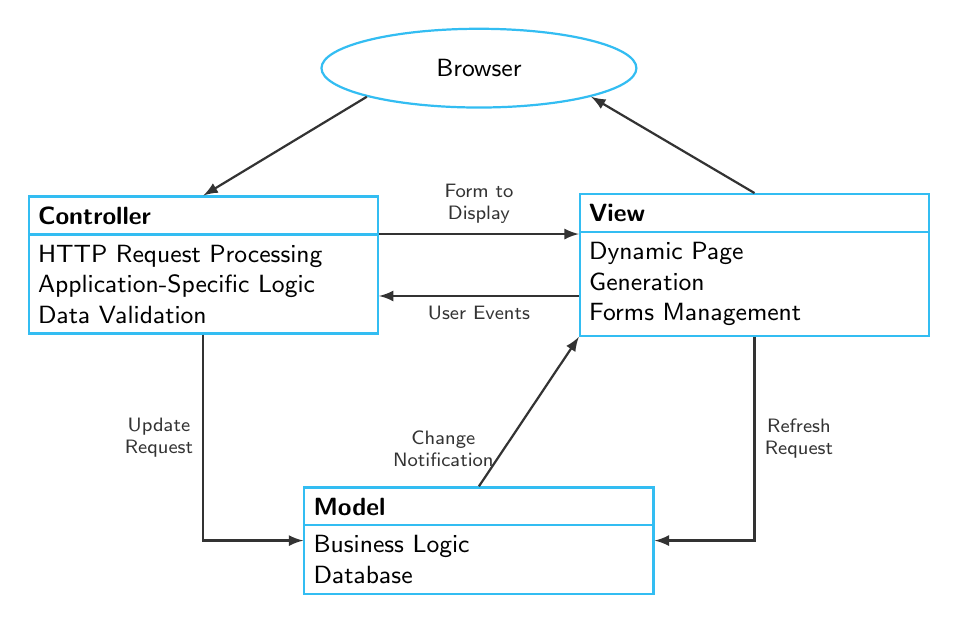
\begin{tikzpicture}[
        node distance=3cm and 4cm,
        mvcbox/.style={
            rectangle split, rectangle split parts=2,
            draw=cyan!80, thick, fill=white,
            rectangle split part fill={cyan!80, white},
            minimum width=4cm, align=left, font=\small
        },
        browser/.style={ellipse, draw=cyan!80, thick, fill=white, minimum width=4cm, minimum height=1cm, align=center, font=\small},
        arrow/.style={->, >=latex, thick, black!80}
    ]
        
        % Browser
        \node[browser] (browser) at (0, 2.5) {Browser};

        % Controller
        \node[mvcbox, text width=4.2cm] (ctrl) at (-3.5, 0) {
            \nodepart{one} \centering \textbf{Controller}
            \nodepart{two} 
            HTTP Request Processing\\
            Application-Specific Logic\\
            Data Validation
        };

        % View
        \node[mvcbox, text width=4.2cm] (view) at (3.5, 0) {
            \nodepart{one} \centering \textbf{View}
            \nodepart{two} 
            Dynamic Page\\
            Generation\\
            Forms Management
        };

        % Model
        \node[mvcbox, text width=4.2cm] (model) at (0, -3.5) {
            \nodepart{one} \centering \textbf{Model}
            \nodepart{two} 
            Business Logic\\
            Database
        };

        % Arrows
        \draw[arrow] (browser.south west) -- (ctrl.north);
        \draw[arrow] (view.north) -- (browser.south east);
        
        % Controller <-> View
        \draw[arrow] (ctrl.10) -- node[above, align=center, font=\scriptsize] {Form to\\Display} (view.170);
        \draw[arrow] (view.190) -- node[below, font=\scriptsize] {User Events} (ctrl.350);

        % Controller -> Model
        \draw[arrow] (ctrl.south) |- node[near start, left, align=center, font=\scriptsize] {Update\\Request} (model.west);

        % Model <-> View
        \draw[arrow] (model.north) -- node[near start, left, align=center, font=\scriptsize] {Change\\Notification} (view.south west);
        \draw[arrow] (view.south) |- node[near start, right, align=center, font=\scriptsize] {Refresh\\Request} (model.east);

    \end{tikzpicture}
    }
\end{frame}

\begin{frame}[fragile]
    \frametitle{Pattern 3: Client-Server Architecture}
    A distributed architecture that partitions tasks between providers of a resource or service (servers) and service requesters (clients).
    
    \vspace{0.2cm}
    \begin{center}
    \resizebox{0.9\textwidth}{!}{
    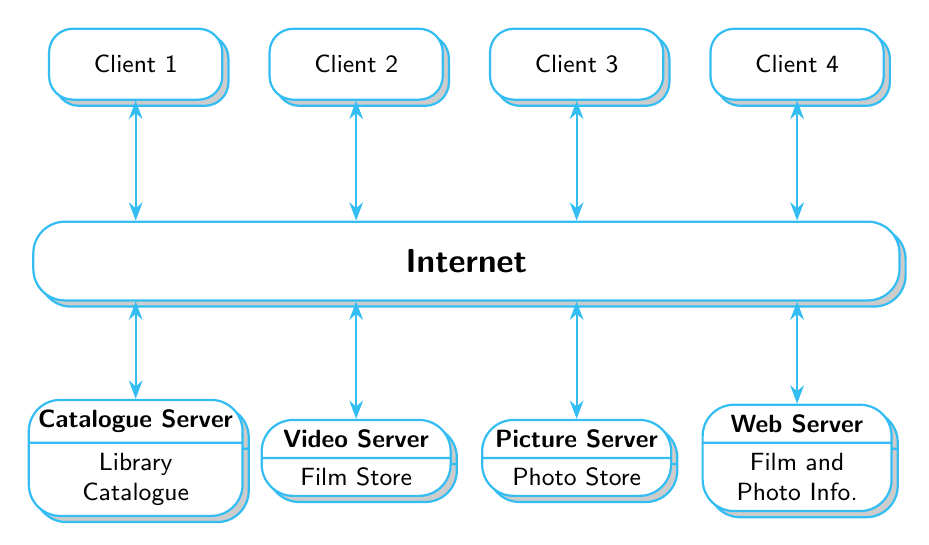
\begin{tikzpicture}[
        client/.style={rectangle, draw=cyan!80, thick, fill=white, rounded corners=3mm, minimum width=2.2cm, minimum height=0.9cm, align=center, font=\small\sffamily, copy shadow={fill=gray!40, shadow xshift=0.5ex, shadow yshift=-0.5ex}},
        server/.style={rectangle split, rectangle split parts=2, draw=cyan!80, thick, fill=white, rounded corners=4mm, minimum width=2.4cm, align=center, font=\small\sffamily, copy shadow={fill=gray!40, shadow xshift=0.5ex, shadow yshift=-0.5ex}},
        network/.style={rectangle, draw=cyan!80, thick, fill=white, rounded corners=4mm, minimum width=11cm, minimum height=1cm, align=center, font=\large\sffamily\bfseries, copy shadow={fill=gray!40, shadow xshift=0.5ex, shadow yshift=-0.5ex}},
        arrow/.style={<->, >=Stealth, thick, cyan!80}
    ]
        
        % The Internet
        \node[network] (net) at (0, 0) {Internet};
        
        % Clients (top row)
        \node[client] (c1) at (-4.2, 2.5) {Client 1};
        \node[client] (c2) at (-1.4, 2.5) {Client 2};
        \node[client] (c3) at (1.4, 2.5) {Client 3};
        \node[client] (c4) at (4.2, 2.5) {Client 4};
        
        % Servers (bottom row)
        \node[server] (s1) at (-4.2, -2.5) {\textbf{Catalogue Server}\nodepart{two}Library\\Catalogue};
        \node[server] (s2) at (-1.4, -2.5) {\textbf{Video Server}\nodepart{two}Film Store};
        \node[server] (s3) at (1.4, -2.5) {\textbf{Picture Server}\nodepart{two}Photo Store};
        \node[server] (s4) at (4.2, -2.5) {\textbf{Web Server}\nodepart{two}Film and\\Photo Info.};
        
        % Connections to network
        \draw[arrow] (c1.south) -- (c1.south |- net.north);
        \draw[arrow] (c2.south) -- (c2.south |- net.north);
        \draw[arrow] (c3.south) -- (c3.south |- net.north);
        \draw[arrow] (c4.south) -- (c4.south |- net.north);
        
        \draw[arrow] (s1.north) -- (s1.north |- net.south);
        \draw[arrow] (s2.north) -- (s2.north |- net.south);
        \draw[arrow] (s3.north) -- (s3.north |- net.south);
        \draw[arrow] (s4.north) -- (s4.north |- net.south);

    \end{tikzpicture}
    }
    \end{center}
\end{frame}

%------------------------------------------------------------
\section{Design Patterns}
%------------------------------------------------------------

\begin{frame}
    \frametitle{Design Patterns}
    \begin{block}{Definition}
        A design pattern is a general, reusable solution to a commonly occurring problem within a given context in software design.
    \end{block}
    \vspace{0.3cm}
    \textbf{Key Characteristics:}
    \begin{itemize}
        \item It is not a finished design that can be directly transformed into code.
        \item It is a template for how to solve a problem that can be used in many different situations.
        \item It describes the problem, the solution, and the consequences of using that solution.
    \end{itemize}
\end{frame}

\begin{frame}
    \frametitle{Design Patterns}
        \begin{columns}
            \column{0.5\textwidth}
            The Gang of Four (GoF) Design Patterns refer to a set of 23 classic software design patterns, documented in the highly influential 1994 book.
            \vspace{0.5cm}

            The book quickly became a cornestone of object-oriented design, and the patterns it describes are still widely used today.
            \column{0.5\textwidth}
            \begin{center}
                
\includegraphics[width=0.9\textwidth]{imgs/designpatterns.png}
            \end{center}
            % \vspace{0.1cm}
            \tiny\textit{Available at the library.}
        \end{columns}

\end{frame}

\begin{frame}
    \frametitle{Architecture vs. Design Patterns}
    \begin{itemize}
        \item \textbf{Architectural Patterns} deal with the high-level organization of your entire software system (e.g., MVC).
        \item \textbf{Design Patterns} are used at a lower level to solve recurring problems at the code/class construction level.
    \end{itemize}
    \vspace{0.3cm}
    \textbf{The "Gang of Four" (GoF) Categories:}
    \begin{enumerate}
        \item \textbf{Creational:} How objects are created (e.g., Singleton, Factory).
        \item \textbf{Structural:} How objects are composed (e.g., Facade, Adapter).
        \item \textbf{Behavioral:} How objects communicate (e.g., Observer, Iterator).
    \end{enumerate}
\end{frame}

\begin{frame}[fragile]
    \frametitle{1. Creational: The Singleton Pattern}
    \textbf{Problem:} You need exactly *one* instance of a class across the entire application (e.g., a Database Connection, or a Robot API Client).
    
    \vspace{0.2cm}
    \begin{columns}
        \column{0.45\textwidth}
        \textbf{Solution:}
        Make the constructor private. Provide a static method that creates the instance only if it doesn't exist yet, and returns the existing one if it does.
        
        \column{0.55\textwidth}
        \centering
        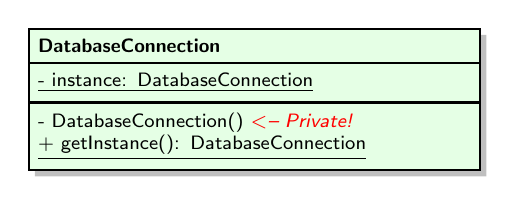
\begin{tikzpicture}[
            classbox/.style={
                rectangle split, rectangle split parts=3, 
                draw=black, fill=green!10, thick, 
                text width=5.5cm, align=left, 
                font=\scriptsize, drop shadow
            }
        ]
            \node[classbox] (sing) {
                \nodepart{one} \centering \textbf{DatabaseConnection}
                \nodepart{two} 
                \underline{- instance: DatabaseConnection}
                \nodepart{three}
                - DatabaseConnection() \textcolor{red}{\textit{$<$-- Private!}}\\
                \underline{+ getInstance(): DatabaseConnection}
            };
        \end{tikzpicture}
    \end{columns}
    \vspace{0.4cm}
    \textit{Note: The underline in UML means a property/method is Static.}
\end{frame}

\begin{frame}[fragile]
    \frametitle{2. Behavioral: The Observer Pattern}
    \textbf{Problem:} You need to tell several objects that the state of some other object has changed (e.g., updating multiple UI widgets when the Robot's battery drops).
    
    \vspace{0.2cm}
    \centering
    \resizebox{0.9\textwidth}{!}{
    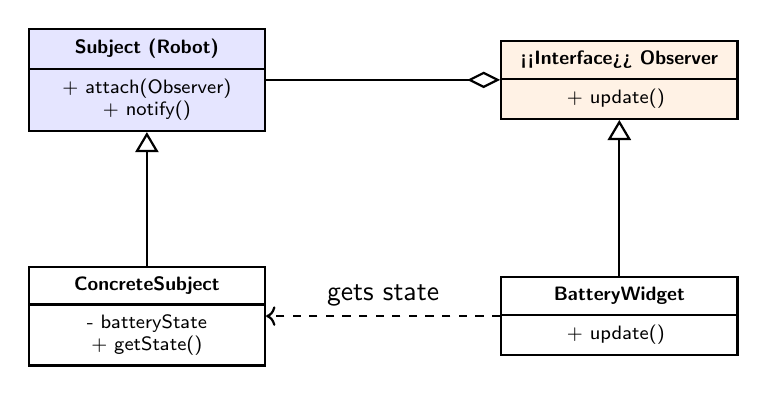
\begin{tikzpicture}[
        classbox/.style={rectangle split, rectangle split parts=2, draw=black, fill=white, thick, minimum width=3cm, align=center, font=\scriptsize},
        inherit/.style={-{Triangle[open, scale=1.5]}, thick},
        agg/.style={-{Diamond[open, scale=1.5]}, thick}
    ]
        \node[classbox, fill=blue!10] (subj) at (0,0) {
            \textbf{Subject (Robot)}
            \nodepart{two} + attach(Observer)\\+ notify()
        };
        \node[classbox, fill=orange!10] (obs) at (6,0) {
            \textbf{<<Interface>> Observer}
            \nodepart{two} + update()
        };
        \node[classbox] (csubj) at (0,-3) {
            \textbf{ConcreteSubject}
            \nodepart{two} - batteryState\\+ getState()
        };
        \node[classbox] (cobs) at (6,-3) {
            \textbf{BatteryWidget}
            \nodepart{two} + update()
        };

        \draw[agg] (subj.east) -- (obs.west);
        \draw[inherit] (csubj.north) -- (subj.south);
        \draw[inherit] (cobs.north) -- (obs.south);
        \draw[->, dashed, thick] (cobs.west) -- (csubj.east) node[midway, above] {gets state};
    \end{tikzpicture}
    }
\end{frame}

\begin{frame}[fragile]
    \frametitle{3. Structural: The Facade Pattern}
    
    
    \textbf{Problem:} You need to "tidy up the interfaces to a number of related objects that have often been developed incrementally". Complex subsystems with many moving parts can overwhelm the client code.
    
    \vspace{0.2cm}
    \begin{columns}
        \column{0.45\textwidth}
        \textbf{Solution:} Provide a unified, simplified, higher-level interface (a "Facade") that makes the subsystem easier to use. The client talks \textit{only} to the Facade, which handles the messy internal delegation.
        
        \column{0.55\textwidth}
        \centering
        \resizebox{\textwidth}{!}{
        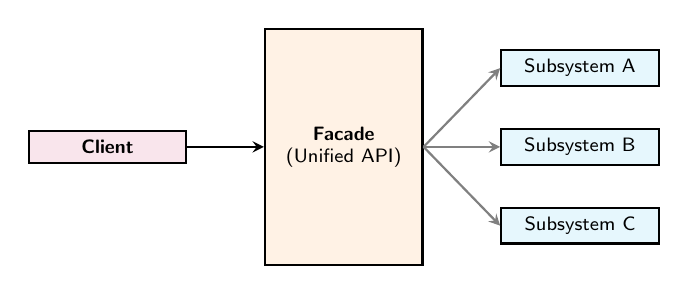
\begin{tikzpicture}[
            box/.style={rectangle, draw=black, fill=white, thick, minimum width=2cm, align=center, font=\scriptsize},
            arrow/.style={->, >=stealth, thick, gray}
        ]
            \node[box, fill=purple!10] (client) at (-2, 0) {\textbf{Client}};
            \node[box, fill=orange!10, minimum height=3cm] (facade) at (1, 0) {\textbf{Facade}\\(Unified API)};
            
            \node[box, fill=cyan!10] (sub1) at (4, 1) {Subsystem A};
            \node[box, fill=cyan!10] (sub2) at (4, 0) {Subsystem B};
            \node[box, fill=cyan!10] (sub3) at (4, -1) {Subsystem C};
            
            \draw[arrow, black] (client) -- (facade);
            \draw[arrow] (facade.east) -- (sub1.west);
            \draw[arrow] (facade.east) -- (sub2.west);
            \draw[arrow] (facade.east) -- (sub3.west);
        \end{tikzpicture}
        }
    \end{columns}
\end{frame}

\begin{frame}
    \frametitle{The Facade Pattern - Example}

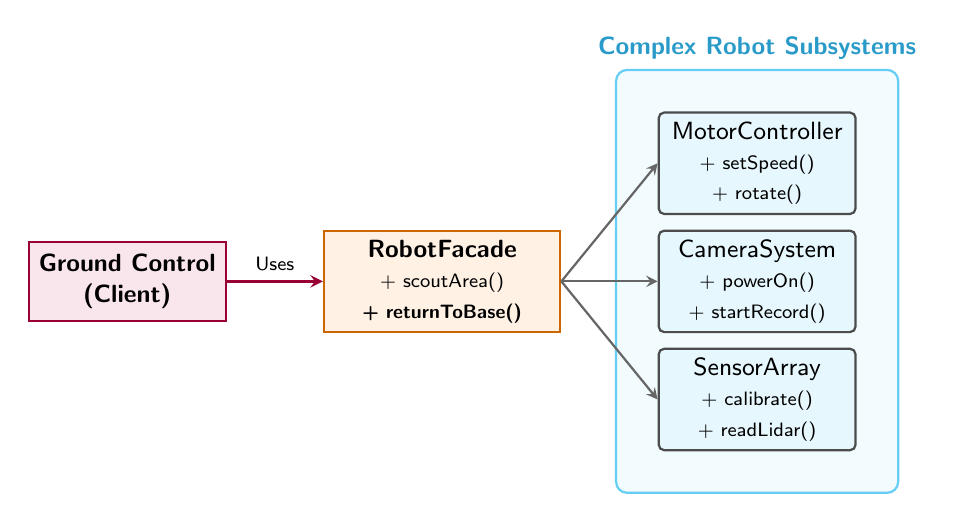
\begin{tikzpicture}[
    % Define styles
    classbox/.style={rectangle, draw=black!70, thick, fill=white, minimum width=2.5cm, minimum height=1cm, align=center, font=\sffamily\small, rounded corners=2pt},
    facadebox/.style={rectangle, draw=orange!80!black, thick, fill=orange!10, minimum width=3cm, minimum height=1.2cm, align=center, font=\sffamily\bfseries\small},
    clientbox/.style={rectangle, draw=purple!80!black, thick, fill=purple!10, minimum width=2.5cm, minimum height=1cm, align=center, font=\sffamily\bfseries\small},
    arrow/.style={->, >=stealth, thick, draw=gray!80!black}
]

    % 1. The Client
    \node[clientbox] (client) at (-4, 0) {Ground Control\\(Client)};

    % 2. The Facade
    \node[facadebox] (facade) at (0, 0) {RobotFacade\\ \normalfont\scriptsize + scoutArea()\\ \scriptsize + returnToBase()};

    % 3. The Complex Subsystems
    \node[classbox, fill=cyan!10] (motor) at (4, 1.5) {MotorController\\ \scriptsize + setSpeed()\\ \scriptsize + rotate()};
    \node[classbox, fill=cyan!10] (camera) at (4, 0) {CameraSystem\\ \scriptsize + powerOn()\\ \scriptsize + startRecord()};
    \node[classbox, fill=cyan!10] (sensor) at (4, -1.5) {SensorArray\\ \scriptsize + calibrate()\\ \scriptsize + readLidar()};

    % Draw a box around the subsystems to show they are a complex group
    \begin{scope}[on background layer]
        \node[rectangle, draw=cyan!60, thick, fill=cyan!5, rounded corners, fit=(motor) (camera) (sensor), inner sep=15pt, label={[font=\sffamily\bfseries\small, text=cyan!80!black]above:Complex Robot Subsystems}] (subsystem_box) {};
    \end{scope}

    % 4. Connections (Arrows)
    % Client talks ONLY to the Facade
    \draw[arrow, draw=purple!80!black, line width=1pt] (client.east) -- (facade.west) node[midway, above, font=\sffamily\scriptsize, text=black] {Uses};

    % Facade manages the messy subsystems
    \draw[arrow] (facade.east) -- (motor.west);
    \draw[arrow] (facade.east) -- (camera.west);
    \draw[arrow] (facade.east) -- (sensor.west);

\end{tikzpicture}

\end{frame}

%------------------------------------------------------------
\section{Software Reuse \& Open Source}
%------------------------------------------------------------

\begin{frame}
    \frametitle{From Reusing Ideas to Reusing Code}
    We just discussed \textbf{Patterns}, which is how we reuse abstract knowledge and design solutions. But what if we want to reuse actual, compiled code?
    
    \vspace{0.3cm}
    \textbf{Most modern software is constructed by reusing existing components or systems rather than writing everything from scratch.}
\end{frame}

\begin{frame}
    \frametitle{The Reuse Landscape}
    
    \begin{block}{Levels of Reuse}
        \begin{itemize}
            \item \textbf{Abstraction Level:} Reusing knowledge (Design/Architectural Patterns).
            \item \textbf{Object/Function Level:} Reusing libraries (e.g., Python's \texttt{math} or \texttt{datetime}).
            \item \textbf{Component Level:} Reusing frameworks (e.g., React.js for UI, Express.js for routing).
            \item \textbf{System Level:} Reusing entire applications (e.g., integrating MySQL or a Virtual Docker container).
        \end{itemize}
    \end{block}
\end{frame}

\begin{frame}
    \frametitle{Benefits \& Risks of Software Reuse}
    
    
    \rowcolors{2}{gray!10}{white}
    \begin{table}
        \centering
        \scriptsize
        \begin{tabular}{|p{0.45\textwidth}|p{0.45\textwidth}|}
            \hline
            \rowcolor{cyan!20}
            \textbf{Benefits} & \textbf{Problems} \\
            \hline
            \textbf{Accelerated Development:} Bringing a system to market early is often more important than overall development costs. & \textbf{Lack of Trust / Not-Invented-Here:} Developers often prefer to rewrite components because they believe they can improve on them. \\
            \textbf{Increased Dependability:} Reused software that has been tried and tested should be more dependable than new software. & \textbf{Maintenance \& Dependencies:} If a reused component breaks or loses support, your system breaks. \\
            \hline
        \end{tabular}
    \end{table}
    
    \vspace{0.2cm}
    \footnotesize \textbf{Real-World Example:} In 2016, a developer deleted an 11-line open-source component called \texttt{left-pad} from the NPM registry. Because thousands of other components depended on it, large parts of the global internet (including React and Node) temporarily broke!
\end{frame}

\begin{frame}
    \frametitle{Open-Source Development}
    Today, the primary vehicle for Software Reuse is \textbf{Open-Source Development}.
    
    \begin{itemize}
        \item \textbf{What is it?} An approach where the source code of a software system is published, and volunteers are invited to participate in the development process.
        \item \textbf{Roots:} Started by the Free Software Foundation, advocating that source code should not be proprietary.
        \item \textbf{Scale:} Extended by the Internet to recruit massive populations of volunteer developers and users.
    \end{itemize}
    
    \vspace{0.2cm}
    \textbf{Famous Real-World Examples:} The Linux operating system, Apache web server, and MySQL database management system are massively successful open-source products.
\end{frame}

\begin{frame}
    \frametitle{Open-Source Licensing (The LEPSI Connection)}
    
    
    Just because source code is freely available does \textbf{not} mean you can do whatever you want with it. The developer legally owns the code and places restrictions via licenses.
    
    \vspace{0.2cm}
    \begin{block}{Permissive Licenses (e.g., MIT, Apache 2.0)}
        Allow you to license your project however you want, even in closed-source, proprietary, for-profit products.
    \end{block}
    
    \begin{alertblock}{Copyleft Licenses (e.g., GPLv2, GPLv3)}
        "Strong" copyleft. Including any library with these licenses requires you to choose an identical or compatible license for your entire project.
    \end{alertblock}
    
    % \vspace{0.1cm}
    % \footnotesize \textbf{Real-World Example:} Cisco/Linksys used Linux (GPL) in their WRT54G routers. They were sued and legally forced to release their router firmware's source code to the public, spawning the massive open-source DD-WRT router community!
\end{frame}
%------------------------------------------------------------
\section{Component-Based Software Engineering}
%------------------------------------------------------------


\begin{frame}
    \frametitle{Introduction to CBSE}
    We have seen how to reuse abstract knowledge (Patterns) and how the industry shares reusable code (Open Source). But how do we architect systems to ensure this reused code integrates flawlessly?
    
    \vspace{0.2cm}
    \begin{block}{Component-Based Software Engineering (CBSE)}
        An approach to software development that relies on the reuse of entities called 'software components'.
    \end{block}
    \small
    \begin{itemize}
        \item It emerged from the failure of object-oriented development to support effective reuse. Single object classes are too detailed and specific.
        \item Components are more abstract than object classes and act as stand-alone service providers.
        \item They can exist as independent, executable entities.
    \end{itemize}
\end{frame}

\begin{frame}[fragile]
    \frametitle{CBSE Interfaces (The General Form)}
    
    
    The services offered by a component are made available through an interface, and all interactions take place through that interface. We model this using UML "ball and socket" notation.
    
    \vspace{0.3cm}
    \centering
    \resizebox{0.9\textwidth}{!}{
    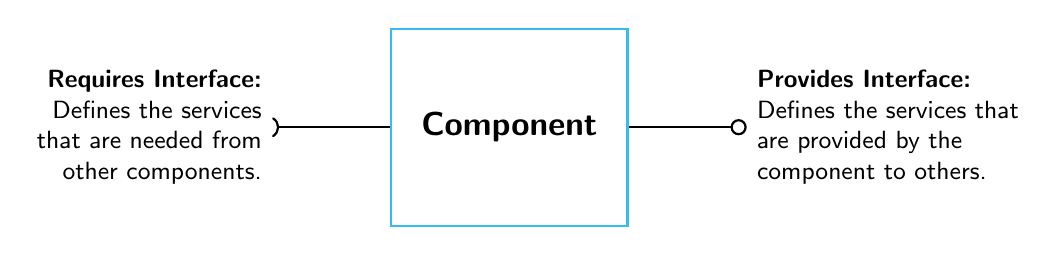
\begin{tikzpicture}[
        comp/.style={rectangle, draw=cyan!80, thick, fill=white, minimum width=3cm, minimum height=2.5cm, align=center, font=\large\bfseries},
        prov/.style={-o, thick},
        req/.style={-(, thick}
    ]
        \node[comp] (c) {Component};
        
        % Provides
        \draw[prov] (c.east) -- +(1.5,0) node[right, align=left, font=\small] {\textbf{Provides Interface:}\\Defines the services that\\are provided by the\\component to others.};
        
        % Requires
        \draw[req] (c.west) -- +(-1.5,0) node[left, align=right, font=\small] {\textbf{Requires Interface:}\\Defines the services\\that are needed from\\other components.};
    \end{tikzpicture}
    }
    
    \vspace{0.3cm}
    \footnotesize \textit{Note: The 'requires' interface does not compromise independence, because it doesn't define \textbf{how} the external service is implemented, only that it is needed.}
\end{frame}

\begin{frame}[fragile]
    \frametitle{CBSE Interfaces (A Concrete Example)}
    Let's look at how this general form applies to a specific subsystem: a \textbf{Data Collector} component.
    
    \vspace{0.2cm}
    \centering
    \resizebox{0.8\textwidth}{!}{
    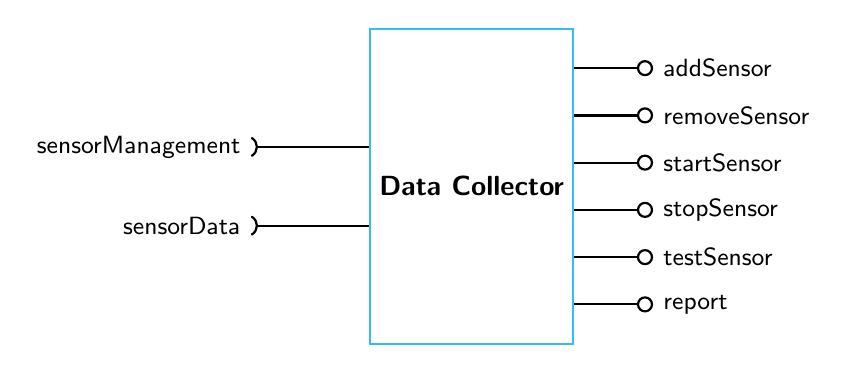
\begin{tikzpicture}[
        comp/.style={rectangle, draw=cyan!80, thick, fill=white, minimum width=2.5cm, minimum height=4cm, align=center, font=\bfseries},
        prov/.style={-o, thick},
        req/.style={-(, thick}
    ]
        \node[comp] (c) {Data Collector};
        
        % Provides
        \draw[prov] ([yshift=1.5cm]c.east) -- +(1,0) node[right, font=\small] {addSensor};
        \draw[prov] ([yshift=0.9cm]c.east) -- +(1,0) node[right, font=\small] {removeSensor};
        \draw[prov] ([yshift=0.3cm]c.east) -- +(1,0) node[right, font=\small] {startSensor};
        \draw[prov] ([yshift=-0.3cm]c.east) -- +(1,0) node[right, font=\small] {stopSensor};
        \draw[prov] ([yshift=-0.9cm]c.east) -- +(1,0) node[right, font=\small] {testSensor};
        \draw[prov] ([yshift=-1.5cm]c.east) -- +(1,0) node[right, font=\small] {report};
        
        % Requires
        \draw[req] ([yshift=0.5cm]c.west) -- +(-1.5,0) node[left, font=\small] {sensorManagement};
        \draw[req] ([yshift=-0.5cm]c.west) -- +(-1.5,0) node[left, font=\small] {sensorData};
    \end{tikzpicture}
    }
    
    \vspace{0.2cm}
    \footnotesize \textit{The Data Collector provides an API to add and start sensors, but it explicitly requires external data and management subsystems to function.}
\end{frame}

\begin{frame}
    \frametitle{Modern CBSE: Services \& Microservices}
    \small
    Historically, CBSE relied on strict component models like Sun's Enterprise Java Beans (EJB), Microsoft's COM+/.NET, and CORBA.
    
    \vspace{0.2cm}
    \begin{alertblock}{The Problem}
        In practice, these standards hindered the uptake of CBSE because it was often impossible for components developed using different approaches to work together.
    \end{alertblock}
    
    \vspace{0.2cm}
    \textbf{The Modern Solution:}
    In response, the notion of \textbf{component as a service} was developed. 
    \begin{itemize}
        \item Service-oriented components are stand-alone entities accessed over a network (e.g., RESTful APIs).
        \item Instead of language-specific standards, the industry adopted \textbf{Microservices} deployed in \textbf{Containerised units} (e.g. using Docker).
        \item You need only to reference the component via an endpoint, rather than importing its entire source code.
    \end{itemize}
\end{frame}

\begin{frame}
    \frametitle{CBSE Processes}
    CBSE processes are software processes that take into account the possibilities of reuse and the different activities involved.
    
    \vspace{0.3cm}
    This splits the engineering workflow into two distinct approaches:
    
    \begin{enumerate}
        \item \textbf{Development FOR Reuse:}
        \begin{itemize}
            \item Concerned with developing components or services that will be reused in other applications.
            \item It usually involves generalizing existing components so they are abstract enough to be helpful to others.
        \end{itemize}
        \vspace{0.2cm}
        \item \textbf{Development WITH Reuse:}
        \begin{itemize}
            \item The process of developing new applications using existing components and services.
            \item Instead of writing from scratch, engineers act as integrators, wiring together databases, API services, and UI frameworks.
        \end{itemize}
    \end{enumerate}
\end{frame}



% \begin{frame}
%     \frametitle{Component-Based Software Engineering (CBSE)}
%     Emerged from the failure of single-object reuse. Components are more abstract; they are stand-alone service providers.
    
%     \vspace{0.2cm}
%     \textbf{Component Interfaces:}
%     \begin{itemize}
%         \item \textbf{Provides Interface:} The API the component offers to others.
%         \item \textbf{Requires Interface:} The external services the component needs to function.
%     \end{itemize}
    
%     \vspace{0.2cm}
%     \centering
%     \begin{tikzpicture}[
%         comp/.style={rectangle, draw=cyan!80, thick, fill=white, minimum width=3cm, minimum height=2cm, align=center},
%         prov/.style={-o, thick},
%         req/.style={-(, thick}
%     ]
%         \node[comp] (c) {Data Collector};
        
%         % Auxiliary coordinates
%         \coordinate (c_east_high) at ($(c.east) + (0, 0.5cm)$);
%         \coordinate (c_west_high) at ($(c.west) + (0, 0.25cm)$);
        
%         % Provides
%         \draw[prov] (c.east) -- +(1,0) node[right, font=\scriptsize] {getSensorData()};
%         \draw[prov] (c_east_high) -- +(1,0) node[right, font=\scriptsize] {startSensor()};
        
%         % Requires
%         \draw[req] (c_west_high) -- +(-1,0) node[left, font=\scriptsize] {DB Connection};
%     \end{tikzpicture}
% \end{frame}


% \begin{frame}
%     \frametitle{Modern CBSE: Microservices \& Containers}
%     Historically, CBSE relied on complex standards (CORBA, Java Beans) which hindered adoption because they couldn't talk to each other easily.
    
%     \vspace{0.3cm}
%     \textbf{The Modern Equivalent:}
%     Today, we treat components as \textbf{Services} communicating over standard web protocols (HTTP/REST).
%     \begin{itemize}
%         \item Instead of strict language models, we use \textbf{Docker Containers}.
%         \item This allows a Python backend to easily communicate with a Node.js frontend and a C++ Virtual Robot.
%         \item \textit{Your Assessment 1 project is essentially a modern CBSE architecture!}
%     \end{itemize}
% \end{frame}

%------------------------------------------------------------
\section{Next Steps}
%------------------------------------------------------------

% \begin{frame}
%     \frametitle{This Week's Lab: Applying Patterns}
%     In the workshop, you will move from modeling to implementation by applying these patterns to your Assessment codebase.
    
%     \begin{itemize}
%         \item \textbf{Task 1: The Singleton Config:} Implement a Singleton pattern to manage your backend's connection to the Robot API.
%         \item \textbf{Task 2: MVC Structure:} Organize your frontend code using the Model-View-Controller pattern.
%         \item \textbf{Task 3: License Audit:} Conduct a dependency audit of your libraries to ensure LEPSI compliance.
%     \end{itemize}
% \end{frame}

\begin{frame}
    \frametitle{Reading \& Resources}
    \begin{itemize}
        \item \textbf{Recommended Reading:} 
        Sommerville, \textit{Software Engineering 9th Edition}, Chapters 6, 7, 16, and 17.\\ AND\\the original "Gang of Four" book: Gamma et al., \textit{Design Patterns: Elements of Reusable Object-Oriented Software}.
        \item \textbf{\href{https://refactoring.guru/design-patterns}{refactoring.guru/design-patterns}:} An interactive resource for learning Design Patterns with code examples in Python, Java, C\#, and TS.
        \item \textbf{\href{https://choosealicense.com}{ChooseALicense.com}:} GitHub's guide to understanding open-source licenses.
    \end{itemize}
\end{frame}

\begin{frame}
    \frametitle{Next Week}
    \begin{center}
     \textbf{Next Week:} Human-Computer Interaction 
    \end{center}
\end{frame}

\begin{frame}
    \frametitle{Q \& A}
    \begin{center}
        \Huge Any Questions?\\\vspace{0.5cm} 
        \normalsize fdelduchetto@lincoln.ac.uk
    \end{center}
\end{frame}

\end{document}